\documentclass{standalone}

\usepackage{tikz}
\usetikzlibrary{shapes}
\usetikzlibrary{arrows}
\usetikzlibrary{positioning}

\begin{document}
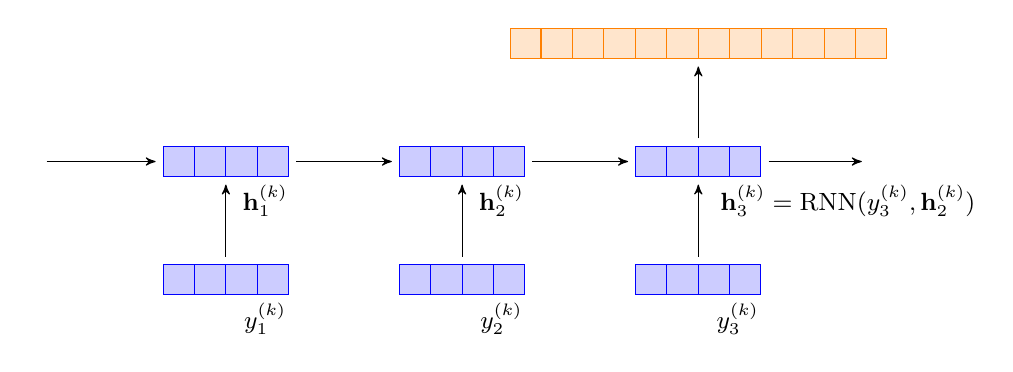
\begin{tikzpicture}[
  hid/.style 2 args={rectangle split, rectangle split horizontal, draw=#2, rectangle split parts=#1, fill=#2!20, outer sep=1mm},
  label/.style={font=\small}]
    \tikzset{>=stealth',every on chain/.append style={join},
      every join/.style={->}}  

  \foreach \step in {1,2,3}
    \node[hid={4}{blue}] (h\step) at (3*\step, 0) {};

  \foreach \step in {1,2,3}
    \node[hid={4}{blue}] (w\step) at (3*\step, -1.5) {};    
    
  \foreach \step in {1,2,3}
    \draw[->] (w\step.north) -> (h\step.south);

  \foreach \step/\next in {1/2,2/3}
    \draw[->] (h\step.east) -> (h\next.west);

  %% edge cases
   \node[] (h0) at (0.6, 0) {};
   \node[] (h4) at (11.2, 0) {};
    \draw[->] (h0.east) -> (h1.west);
    \draw[->] (h3.east) -> (h4.west);
 
  %% make output
  \node[hid={12}{orange}] (o3) at (9, 1.5) {};
  
  \draw[->] (h3.north) -> (o3.south);

  %% labels
  \foreach \step in {1,2}
    \node[label] (hlabel\step) at (3*\step+0.5, -0.5) {$\mathbf{h}_\step^{(k)}$};    
    
 \node[label] (hlabel3) at (10.9, -0.5){$\mathbf{h}_3^{(k)} = \mathrm{RNN}(y_3^{(k)}, \mathbf{h}_2^{(k)})$};

  \foreach \step in {1,2,3}
    \node[label] (wlabel\step) at (3*\step+0.5, -2) {$y_\step^{(k)}$};
        
\end{tikzpicture}
\end{document}